%%=============================================================================
%% Proof of Concept
%%=============================================================================

\chapter{\IfLanguageName{dutch}{Proof of Concept}{Proof of Concept}}%
\label{ch:Proof of Concept}

\section{Doel en Scope}
De Proof of Concept (PoC) heeft als doel aan te tonen hoe een bestaande CI/CD-pipeline kan worden uitgebreid met CRA-relevante securitycontroles, zonder het ontwikkelproces volledig te hertekenen. De focus ligt op twee kernactiviteiten: het genereren van een Software Bill of Materials (SBOM) en het automatisch uitvoeren van dependency scanning met een duidelijke kwaliteitsdrempel (quality gate) op basis van CVSS-scores. Daarnaast werden aanvullende controles geïntegreerd, zoals SAST, container image scanning, secrets scanning en DAST, om een volledig productiewaardige DevSecOps-pipeline te verkrijgen. Dit vormt een referentie-implementatie die door Excentis-teams kan worden overgenomen en in bestaande ontwikkelworkflows kan worden geïntegreerd.

De PoC is bewust beperkt gehouden tot een paar projectrepositories met relatief eenvoudige buildketens (zoals Maven-, .NET- of Python-projecten). Complexere scenario's zoals multi-repo orkestratie of geavanceerde policy engines vallen hier buiten de scope van deze bachelorproef.

\section{Gebruikte tools en omgeving}

\subsection{Gekozen tools}

De implementatie van de Proof of Concept maakt gebruik van Jenkins als CI/CD-platform, aangezien dit reeds binnen Excentis wordt toegepast. Voor de verschillende securiytaken werden uitsluitend open source tools gebruikt:
\begin{itemize}
    \item \textbf{Syft}: SBOM-generatie in CycloneDX-formaat (\texttt{sbom.cdx.json})
    \item \textbf{OWASP Dependency-Check}: Software Composition Analysis (SCA) op basis van NVD-data.
    \item \textbf{SonarQube Community Edition}: Static Application Security Testing (SAST) en codekwaliteit.
    \item \textbf{Grype}: Container image scanning op kwetsbaarheden.
    \item \textbf{TruffleHog}: Secrets scanning op repository en filesystem.
    \item \textbf{OWASP ZAP}: Dynamic Application Security Testing (DAST) op een daaiende container.
\end{itemize}

\subsection{Opzet van de testomgeving}

De PoC is opgezet in een Virtuele Machine (VM) waar een Jenkins Docker container op draait, zodat de integratie van securitystappen zo realistisch mogelijk is. De volgende componenten worden gebruikt:
\begin{itemize}
    \item Een Jenkins Docker-container met toegang tot Docker op de host, zodat images gebouwd en gescand kunnen worden.
    \item Een demo-applicatie (Spring Petclinic) met externe dependencies om realistische SBOMs en dependency-rapporten te kunnen genereren.
    \item Toegang tot het internet voor het downloaden van Syft, Grype, TruffleHog en OWASP ZAP. 
    \item Jenkins-credentials voor een NVD API-key en een Gmail-account voor email notificaties.
\end{itemize}

Alle pipelineconfiguratie is opgeslagen in een \texttt{Jenkinsfile}, zodat wijzigingen in de beveiligingslogica versiebeheer doorlopen zoals gewone broncode.


\section{High-level pipeline-overzicht}

De pipeline volgt een klassieke CI/CD-volgorde waarin de securitystappen zijn geïntegreerd als kwaliteitscontroles (zie Figuur~\ref{fig:pipleine-structuur}). Na codewijzigingen wordt de applicatie opgebouwd en getest en in een containerimage verpakt. Vervolgens worden in parallel meerdere securityflows uitgevoerd: SBOM-generatie en -validatie, dependency scanning, SAST, container image scanning en secrets scanning. Daarna wordt de container gestart en onderworpen aan een DAST-scan met OWASP ZAP. Indien één van de kwaliteitsdrempels wordt overschreden, faalt de pipeline en worden de resultaten als rapporten in Jenkins gepubliceerd.

Deze opbouw zorgt ervoor dat securitycontroles niet losstaan van het ontwikkelproces, maar deel uitmaken van dezelfde geautomatiseerde workflow. Op die manier wordt feedback voor ontwikkelaars vroeg in het proces gegeven en blijft de impact op de bestaande werkwijze beperkt.

\begin{figure}[h]
    \centering
    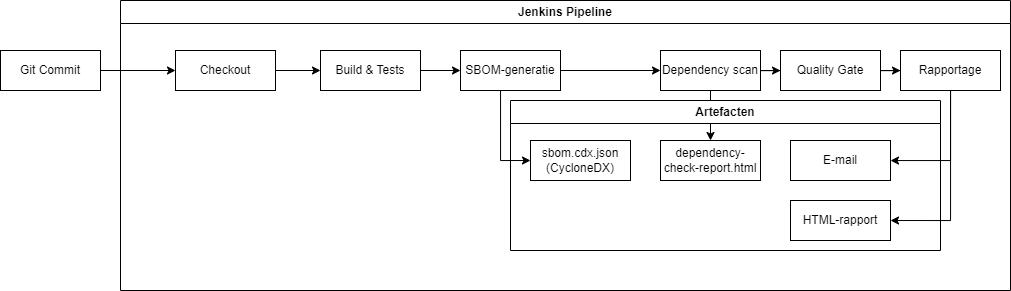
\includegraphics[width=\textwidth]{../graphics/pipeline-structuur.png}
    \caption{Structuur van een CRA-compliant CI/CD-pijplijn.}
    \label{fig:pipleine-structuur}
\end{figure}

\subsection{Pipeline stages}

De pipeline bestaat uit zes opeenvolgende stages die een klassieke CI/CD-workflow combineren met CRA-relevante securitycontroles:

\begin{enumerate}
    \item \textbf{Checkout}: De broncode van Spring Petclinic wordt opgehaald uit de GitHub-repository, zodat de pipeline toegang heeft tot de nieuwste wijzigingen.
    \item \textbf{Maven Build}: De Java-applicatie wordt gecompileerd met Maven (\texttt{mvn clean package -DskipTests}), wat een JAR-bestand in de \texttt{target}-map oplevert.
    \item \textbf{Build Container Image}: Een Docker-image wordt gebouwd op basis van de gecompileerde applicatie en een Dockerfile uit de BAP-repository. Het image wordt getagd als \texttt{spring-petclinic:\$\{BUILD\_NUMBER\}}.
    \item \textbf{Parallel Security Checks}: In deze stage worden vijf securityflows parallel uitgevoerd: SBOM Flow, Dependency-Check Flow, SonarQube Flow, Grype Container Scan en TruffleHog Secrets Scan.
    \item \textbf{Run Container}: De eerder gebouwde container wordt gestart op poort 9090, zodat de applicatie beschikbaar is voor DAST.
    \item \textbf{OWASP ZAP Scan}: Een OWASP ZAP-container voert een DAST-scan uit tegen de draaiende applicatie en genereert HTML- en JSON-rapporten.
    \item \textbf{Compliance Rapport}: Een overkoepelend CRA-compliancerapport kan via Jenkins gepubliceerd worden.
    \item \textbf{Archive Artifacts}: SBOMs, rapporten en andere relevante artefacten worden gearchiveerd als auditbewijs.
    \item \textbf{Post Actions}: Bij fouten wordt een e-mail verstuurd, ongeacht de uitkomst worden container en image opgeruimd en de workspace opgeschoond.
\end{enumerate}

\section{Implementatie van de Jenkins-pipeline}

De volledige Jenkinsfile is opgenomen in Codefragment~\ref{lst:jenkinsfile-full} en wordt hieronder functioneel toegelicht.
\subsection{Basisconfiguratie}

De pipeline draait op een generieke Jenkins-agent en definieert een omgevingsvariabele \texttt{IMAGE\_name} die gebruikt wordt om de Docker containerimage uniek te taggen op basis van het buildnummer:

\begin{listing}[h]
    \caption{Basisconfiguratie van de Jenkins-pipeline}
    \label{lst:jenkins-env}
    \begin{minted}{groovy}
    pipeline {
        agent any
    
        environment {
            IMAGE_NAME = "spring-petclinic:${BUILD_NUMBER}"
        }
    
        tools {
            maven 'Maven'
        }
    
        stages {
            // Stages volgen hier...
        }
    }
    \end{minted}
\end{listing}

\subsection{Build-stappen}

De eerste stages implementeren de klassieke CI-stappen:
   
\begin{itemize}
    \item \textbf{Checkout}: haalt de broncode van GitHub.
    \item \textbf{Maven Build}: bouwt de JAR.
    \item \textbf{Build Container Image}: bouwt het Docker-image op basis van de JAR en Dockerfile.
\end{itemize}

\begin{listing}[h]
    \caption{Checkout, build en container image build}
    \label{lst:jenkins-build}
    \begin{minted}{groovy}
    stage('Checkout') {
        steps {
            git url: 'https://github.com/spring-projects/spring-petclinic.git',
                branch: 'main'
            sh 'ls -a'
        }
    }
    
    stage('Maven Build') {
        steps {
            sh '''
                echo "STARTING MAVEN BUILD"
                mvn clean package -DskipTests -q
                echo "BUILD SUCCESS"
            '''
        }
    }
    
    stage('Build Container Image') {
        steps {
            sh '''
                git clone https://github.com/EngelsIlan/BAP.git
                echo "BUILDING DOCKER IMAGE"
                docker build -f BAP/Docker/Dockerfile -t spring-petclinic:${BUILD_NUMBER} .
                docker images | grep spring-petclinic
            '''
        }
    }
    \end{minted}
\end{listing}

\subsection{Parallelle securitycontroles}

De stage \textbf{Parallel Security Checks} groepeert alle securitycontroles in één parallel blok, zodat de totale doorlooptijd van de pipeline beperkt blijft. Binnen deze stage worden vijf flows onderscheden.
\subsubsection{SBOM Flow}

De \textbf{SBOM Flow} genereert en valideert een CycloneDX-SBOM en controleert deze tegen de BSI TR-03183-2-richtlijnen

\begin{listing}[h]
    \caption{SBOM-generatie en validatie met Syft}
    \label{lst:jenkins-sbom-flow}
    \begin{minted}{groovy}
    stage('SBOM Flow') {
        stages {
            stage('Generate SBOM') {
                steps {
                    sh '''
                        echo "GENERATING SBOM WITH SYFT"
    
                        apt-get update -q
                        apt-get install -y jq python3
    
                        curl -sSfL https://raw.githubusercontent.com/anchore/syft/main/install.sh | sh -s -- -b .
    
                        ./syft scan dir:. -o cyclonedx-json > sbom.cdx.json
    
                        echo "=== SBOM Preview ==="
                        cat sbom.cdx.json | jq '.components | length'
                        cat sbom.cdx.json | jq '.components[0:3] | .[] | {name, version}'
                    '''
                }
            }
    
            stage('Validate & Archive SBOM') {
                steps {
                    sh '''
                        echo "VALIDATING SBOM"
                        cat sbom.cdx.json | jq empty
    
                        COMPONENT_COUNT=$(cat sbom.cdx.json | jq '.components | length')
                        echo "Generated SBOM with $COMPONENT_COUNT components"
    
                        if [ "$COMPONENT_COUNT" -eq 0 ]; then
                            echo "ERROR: No components found in SBOM!"
                            exit 1
                        fi
                    '''
                    archiveArtifacts artifacts: 'sbom.cdx.json,target/*.jar', fingerprint: true
                }
            }
    
            stage('SBOM Validatie (BSI TR-03183-2)') {
                steps {
                    catchError(buildResult: 'UNSTABLE', stageResult: 'FAILURE') {
                        sh '''
                            cd BAP
                            git fetch origin
                            git reset --hard origin/main
                            python3 validate_sbom.py ../sbom.cdx.json
                        '''
                    }
                }
            }
        }
    }
    \end{minted}
\end{listing}
    





\subsection{Configuratie van security tools}

\textbf{Syft configuratie} in de Jenkinsfile voor de generatie van een SBOM in JSON formaat:
\begin{listing}[h]
    \caption{Syft SBOM-generatie in Jenkins pipeline}
    \label{lst:syft-jenkins}
    \begin{minted}{groovy}
    stage('SBOM Generation') {
        steps {
            sh '''
                syft packages target/demo-app.jar \\
                    --exclude "platform:java" \\
                    -o cyclonedx-json=sbom.cdx.json
                archiveArtifacts 'sbom.cdx.json'
            '''
        }
    }
    \end{minted}
    \end{listing}

\textbf{OWASP Dependency-Check configuratie} om de SBOM te controleren op CVEs:
\begin{listing}[h]
    \caption{Dependency-Check scan in Jenkins pipeline}
    \label{lst:dependency-jenkins}
    \begin{minted}{groovy}
    stage('Dependency Scan') {
        steps {
            sh '''
                dependency-check \\
                    --project "Demo App" \\
                    --scan "target/" \\
                    --format HTML,JSON \\
                    --out "reports/" \\
                    --suppression "suppressions.xml"
            '''
            archiveArtifacts artifacts: 'reports/**', allowEmptyArchive: true
        }
    }
    \end{minted}
    \end{listing}

\subsection{Quality Gate implementatie}

De quality gate analyseert het scanrapport en blokkeert de pipeline indien er kwetsbaarheden met CVSS-score > 7.0 aanwezig zijn:
\begin{listing}[h]
    \caption{Quality Gate CVSS-controle}
    \label{lst:quality-gate}
    \begin{minted}{groovy}
    stage('Quality Gate') {
        steps {
            script {
                def criticalVulns = sh(
                    script: 'grep -c "CVSS: [7-9]" reports/dependency-check-report.json || true',
                    returnStdout: true
                ).trim()
                
                if (criticalVulns.toInteger() > 0) {
                    error "Kritieke kwetsbaarheden gedetecteerd: ${criticalVulns}"
                }
            }
        }
    }
    \end{minted}
    \end{listing}

Deze implementatie zorgt ervoor dat alleen code zonder hoge of kritieke kwetsbaarheden door de pipeline raakt, terwijl SBOMs automatisch worden gegenereerd en gearchiveerd voor compliance-doeleinden.%De pipeline is geïmplementeerd als een declaratieve Jenkins pipeline met de volgende stages:

%\begin{verbatim}
%pipeline {
%    agent any
%    stages {
%        stage('Checkout') { ... }
%        stage('Build') { ... }
%        stage('SBOM Generation') { 
%            steps {
%                sh 'syft -o cyclonedx-json target/app.jar > sbom.cdx.json'
%            }
%        }
%        stage('Dependency Scan') { 
%            steps {
%                dependencyCheck ...
%            }
%        }
%        stage('Quality Gate') { ... }
%    }
%}
%\end{verbatim}

\section{Technische Uitdagingen}

\subsection{Tool-integratie}

De eerste technische uitdaging, en degene die ook het moeilijkste zal zijn om te implementeren, bij het opzetten van een DevSecOps-pipeline is de integratie van meerdere securitytools in één consistente workflow. Elke tool heeft een specifiek configuratieformaat, authenticatie- en autorisatiemechanismen, en verwacht andere input- en outputformaten (zoals SBOM in CycloneDX, scanraporten in JSON of HTML). Dit verhoogt de complexiteit van de pipelineconfiguratie en maakt foutafhandeling moeilijker wanneer één van de tools faalt.

Bovendien moet er gekozen worden op welk moment in de pipeline SBOM-generatie en kwetsbaarheidsscans worden uitgevoerd. Build-time integratie levert nauwkeurige SBOMs op die overeenkomen met het artefact dat gedeployed wordt, maar vraagt een goede inpassing in bestaande build-scripts (Maven, npm, Docker,...). Als deze tooling niet correct wordt aangeroepen, bestaat het risico op onvolledige SBOMs of ontbrekende scanresultaten, wat de betrouwbaarheid van de hele keten ondermijnt.

\subsection{Performance Overhead}

Het toevoegen van SBOM-generatie en securityscans introduceert onvermijdelijk extra runtime in de CI/CD-pipeline. SBOM-tools moeten alle dependencies analyseren terwijl SCA- en SAST-tools vaak volledige codebases of container-images doorlopen. Zeker bij grotere projecten kan dit minuten toevoegen aan elke build, wat ontwikkelaars ontmoedigt om regelmatig te mergen en pipelines uit te voeren. Het komt er op neer dat hoe meer code en hoe meer dependencies er zijn, hoe langer het duurt voordat de pipeline volledig uitgevoerd is.

Daarnaast kan ook opslag en transport van data een probleem zijn. SBOMs genereren en verwerken voor meerdere services, is veel werk. Afhankelijk van hoe groot de applicatie is en hoeveel dependencies het heeft kan dit gigantisch veel opslag vereisen. Dit moet ook nog eens 10 jaar opgeslagen blijven per versie, dus er moet een oplossing zijn voor lange termijn opslag van de SBOMs \autocite{CRAEvidenceSBOM}.

\subsection{False positives}

Een derde technische uitdaging is het omgaan met false positives in kwetsbaarheidsscans. SCA-tools matchen componenten vaak op basis van naam en versie tegen publiek beschikbare CVE-databases. Bij libraries die bijna dezelfde naam hebben in verschillende ecosystemen of bij slecht onderhouden CPE-gegevens kunnen kwetsbaarheden ten onrechte aan een project worden gekoppeld. Dit resulteert in ruis in de rapporten en extra werk om issues manueel te verifiëren en op te lossen.

Er is ook een andere kant dan de technische impact bij false positives, de procesmatige impact. Als ontwikkelaars continu als "kritiek" gemarkeerde kwetsbaarheden moeten negeren, vermindert het vertrouwen in de tooling en worden waarschuwingen sneller genegeerd. Een robuuste DevSecOps-pipeline moet daarom mechanismen voorzien om onterechte meldingen te onderdrukken, baseline-vergelijkingen te maken en enkel nieuwe of bevestigde kwetsbaarheden als blocking te behandelen.

\subsection{CRA-specifieke gaps}

Hoewel algemene DevSecOps-praktijken goed gedocumenteerd zijn, blijven er specifieke gebrekken voor CRA-conformiteit.

\textbf{Geen standaard CRA-checklists voor pipelines.} Er bestaan wel algemene DevSecOps-checklists, maar geen officiële of gestandaardiseerde CRA-specifieke controlelijsten voor CI/CD-pipelines. Dit dwingt teams om zelf te interpreteren hoe de CRA (zoals SBOM-kwaliteit, vulnerability handling en conformiteitsbewijs) te vertalen naar concrete pipeline-stappen.

\textbf{Onvolwassen SBOM → CVE-automatisering.} Ondanks dat CRA SBOMs vereist om vulnerabilities te identificeren, blijft de koppeling tussen SBOMs en CVE-databases (NVD, EPSS,...) nog experimenteel. Tools zoals SBOM-CVE-Check bestaan, maar vereisen vaak manuele configuratie en missen robuuste integratie met commerciële pipelines. Dit maakt automatische compliance-validatie onbetrouwbaar.


\section{Resultaten van de PoC}
% TODO


\section{Evaluatie van de PoC}
% TODO
